\pdfoutput=1

\documentclass{l4proj}

%
% put any packages here
%
\usepackage{float}
\usepackage{enumitem}
\usepackage{longtable}
\usepackage{listings}
\usepackage{hyperref}
\usepackage{subfiles}
\usepackage{color}


\newcommand{\nc}[1]{\textcolor{magenta}{(\textbf{NC:} #1)}}
\newcommand{\gac}[1]{\textcolor{cyan}{(\textbf{GAC:} #1)}}
\newcommand{\pwt}[1]{\textcolor{blue}{(\textbf{PWT:} #1)}}

\graphicspath{{images}{../images/}}

\begin{document}
\title{On The Scalability of ROS}
\author{Isaac Jordan}
\date{\today}
\maketitle

\begin{abstract}
Robots, distributed systems, and middleware.
\end{abstract}

\educationalconsent
%
%NOTE: if you include the educationalconsent (above) and your project is graded an A then
%      it may be entered in the CS Hall of Fame
%
\tableofcontents
%==============================================================================

\pagenumbering{arabic}
\subfile{sections/introduction}



%\vspace{-7mm}
%\begin{figure}
%\centering
%\includegraphics[height=9.2cm,width=13.2cm]{uroboros.pdf}
%\vspace{-30mm}
%\caption{An alternative hierarchy of the algorithms.}
%\label{uroborus}
%\end{figure}

\chapter{Background}

\subfile{sections/background-part1}

\subfile{sections/background-part2-middleware-overview}

\subfile{sections/background-part3}


\chapter{Experimental Analysis}

\subfile{sections/experiment1}

\subfile{sections/experiment2}

%%%%%%%%%%%%%%%%
%              %
%  APPENDICES  %
%              %
%%%%%%%%%%%%%%%%
\begin{appendices}

\chapter{Experiment 2 Other Graphs}
\label{exp2-appendix-results}

\begin{figure}
\centering
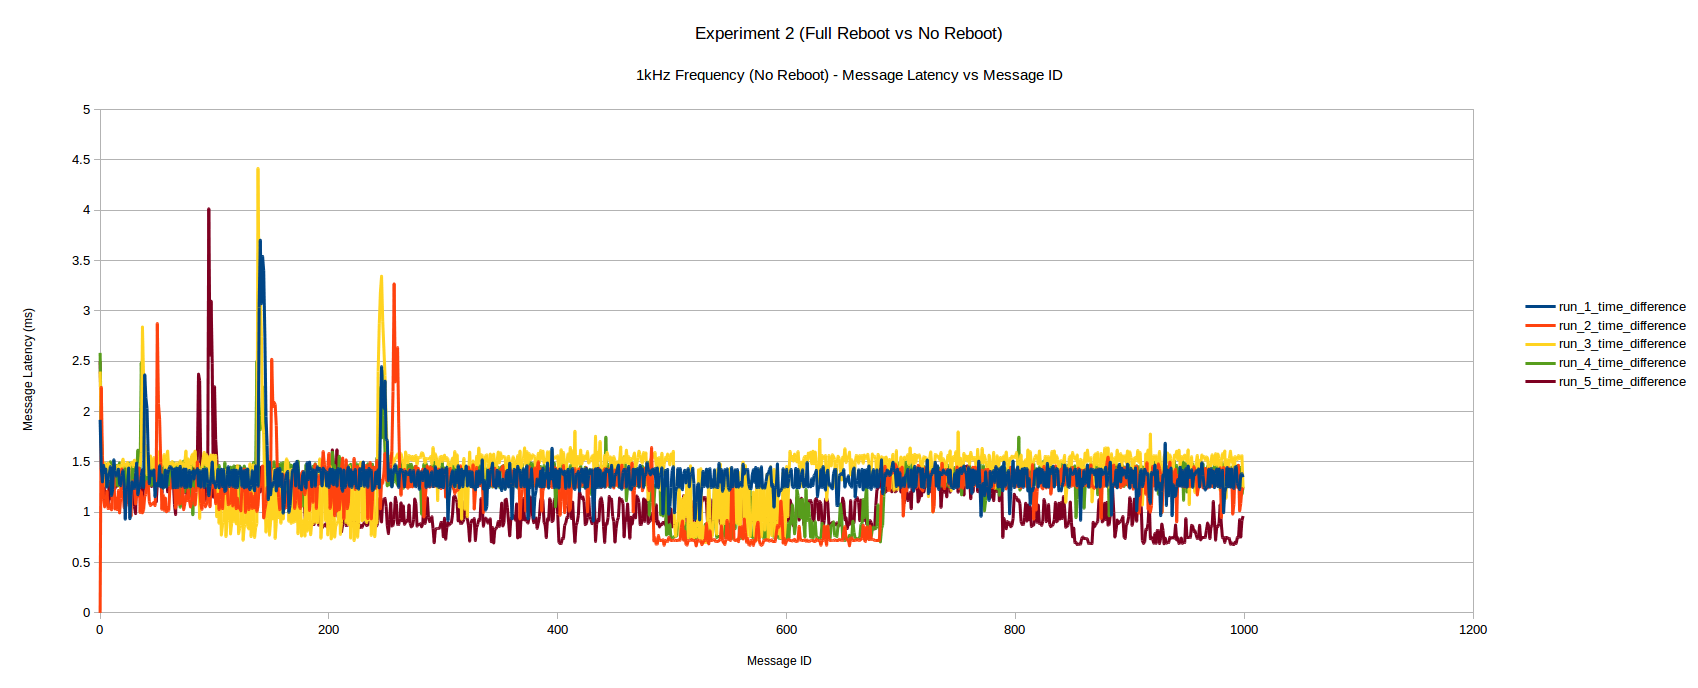
\includegraphics[width=\textwidth]{images/no-reboot-1khz.png}
\caption{Experiment 2 - No Reboot 1KHz Message Frequency}
\label{exp2-noreboot-1khz}
\end{figure}

\begin{figure}
\centering
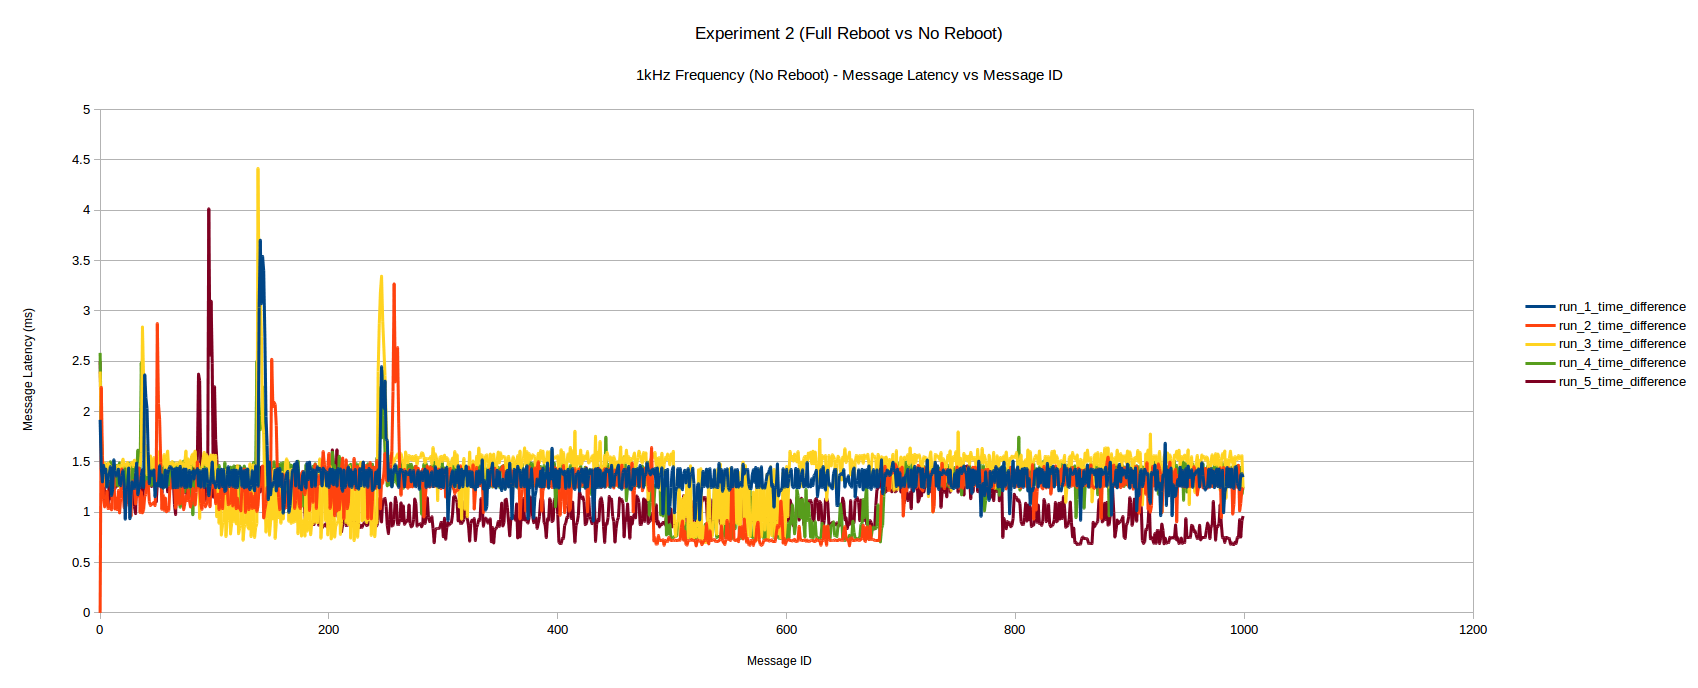
\includegraphics[width=\textwidth]{images/no-reboot-1khz.png}
\caption{Experiment 2 - No Reboot 1KHz Message Frequency}
\label{exp2-fullreboot-1khz}
\end{figure}

\begin{figure}
\centering
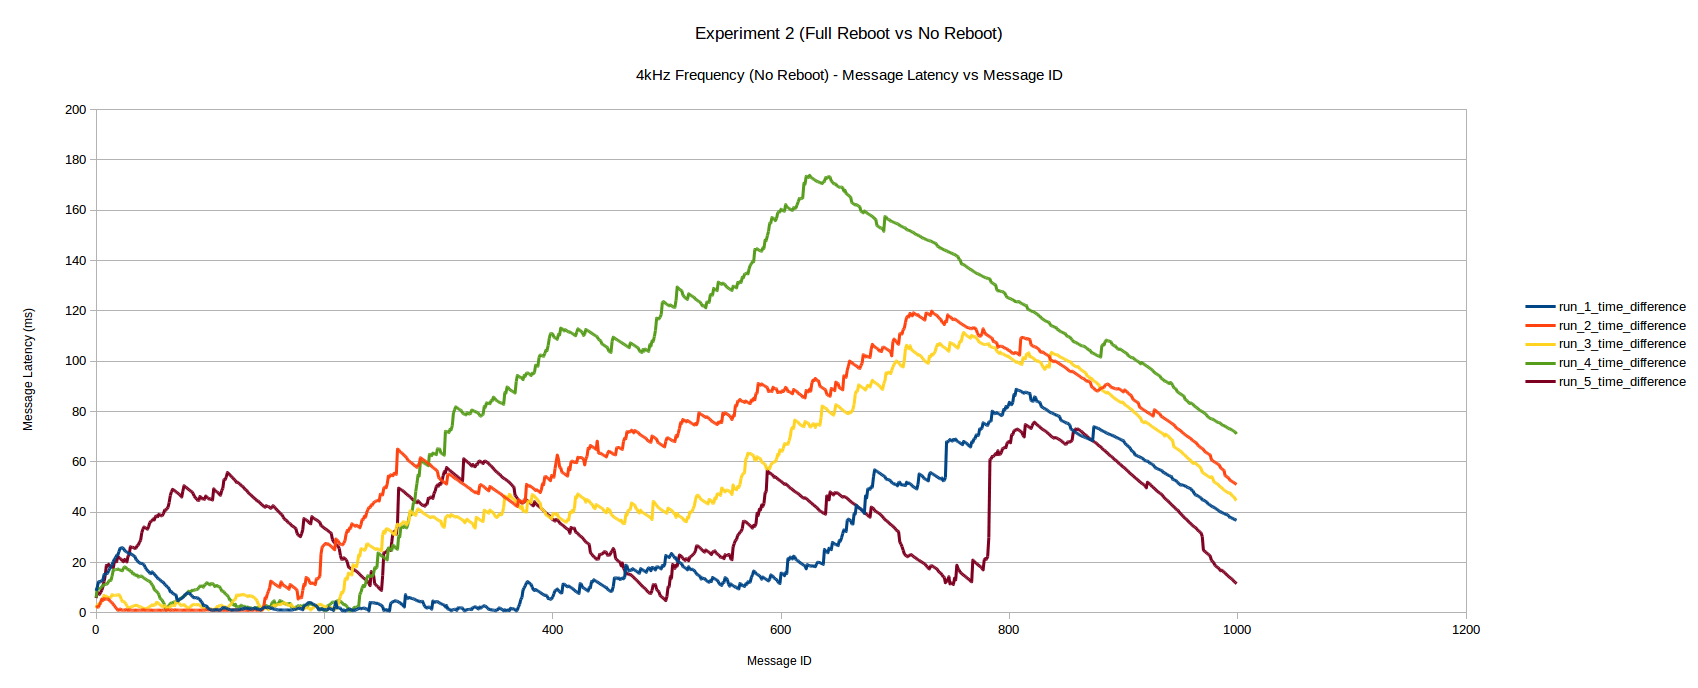
\includegraphics[width=\textwidth]{images/no-reboot-4khz.png}
\caption{Experiment 2 - No Reboot 4KHz Message Frequency}
\label{exp2-noreboot-4khz}
\end{figure}

\begin{figure}
\centering
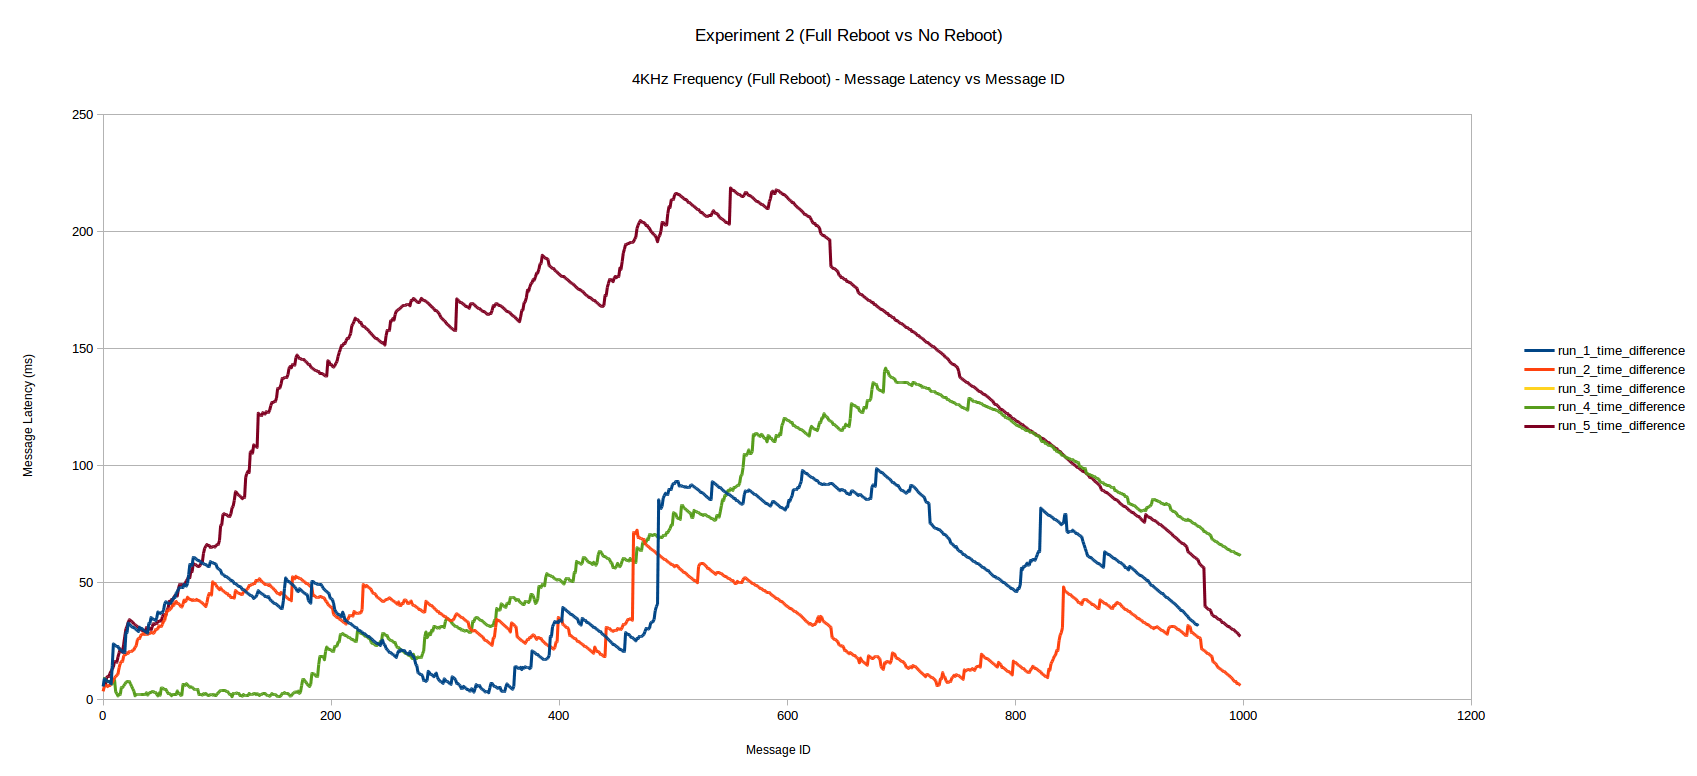
\includegraphics[width=\textwidth]{images/full-reboot-4khz.png}
\caption{Experiment 2 - Full Reboot 4KHz Message Frequency}
\label{exp2-fullreboot-4khz}
\end{figure}

\begin{figure}
\centering
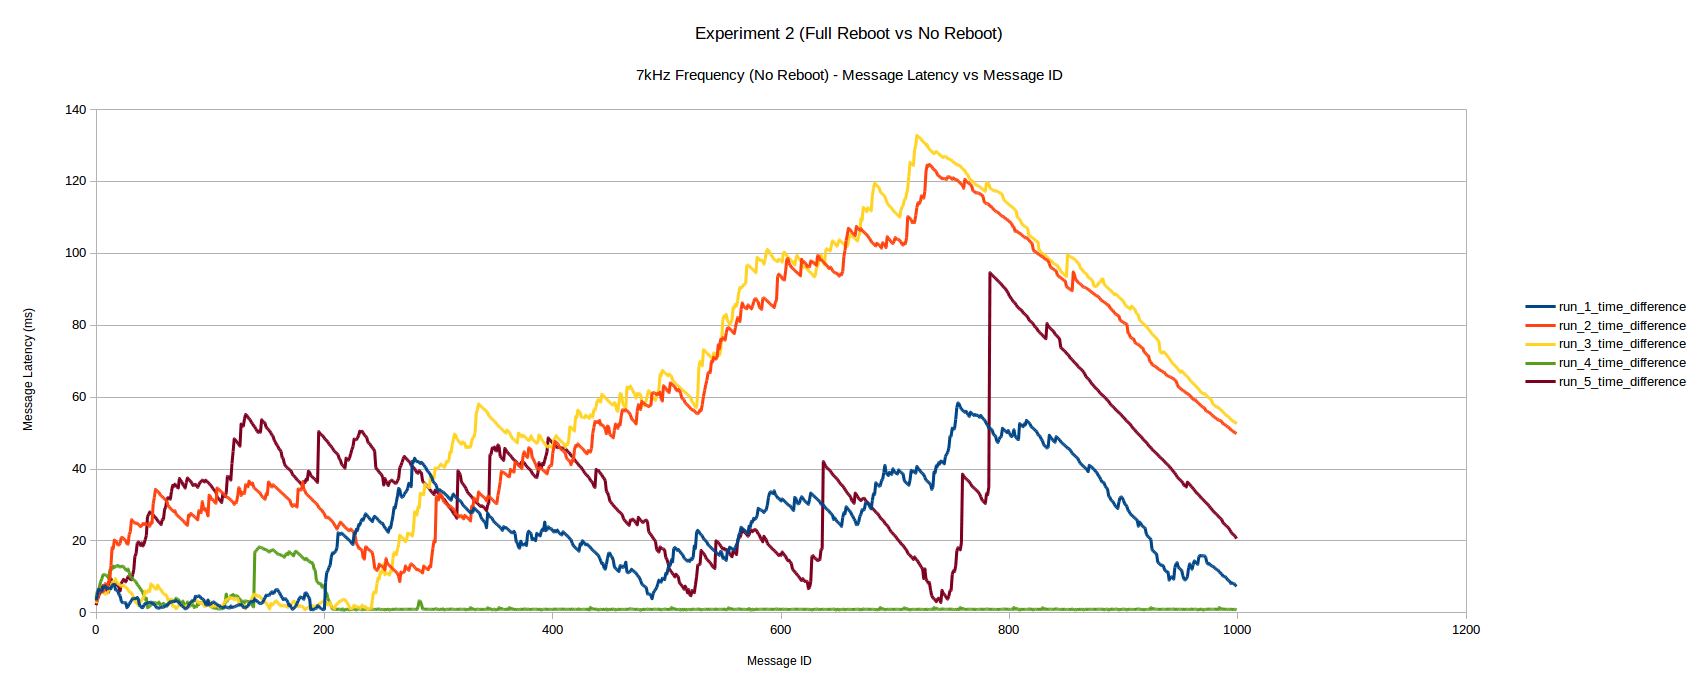
\includegraphics[width=\textwidth]{images/no-reboot-7khz.png}
\caption{Experiment 2 - No Reboot 7KHz Message Frequency}
\label{exp2-noreboot-7khz}
\end{figure}

\begin{figure}
\centering
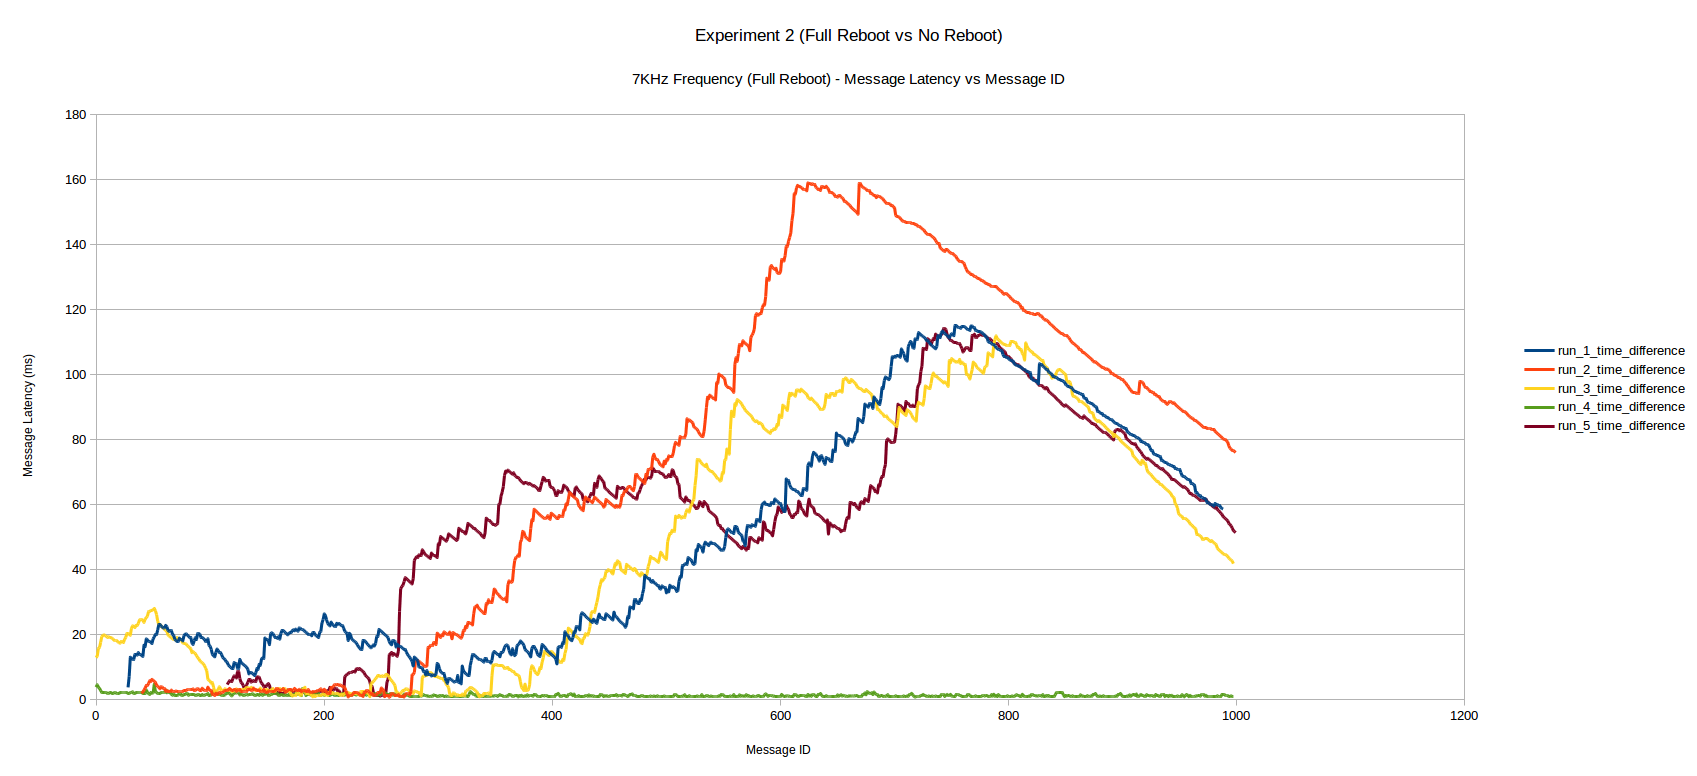
\includegraphics[width=\textwidth]{images/full-reboot-7khz.png}
\caption{Experiment 2 - Full Reboot 7KHz Message Frequency}
\label{exp2-fullreboot-7khz}
\end{figure}

\begin{figure}
\centering
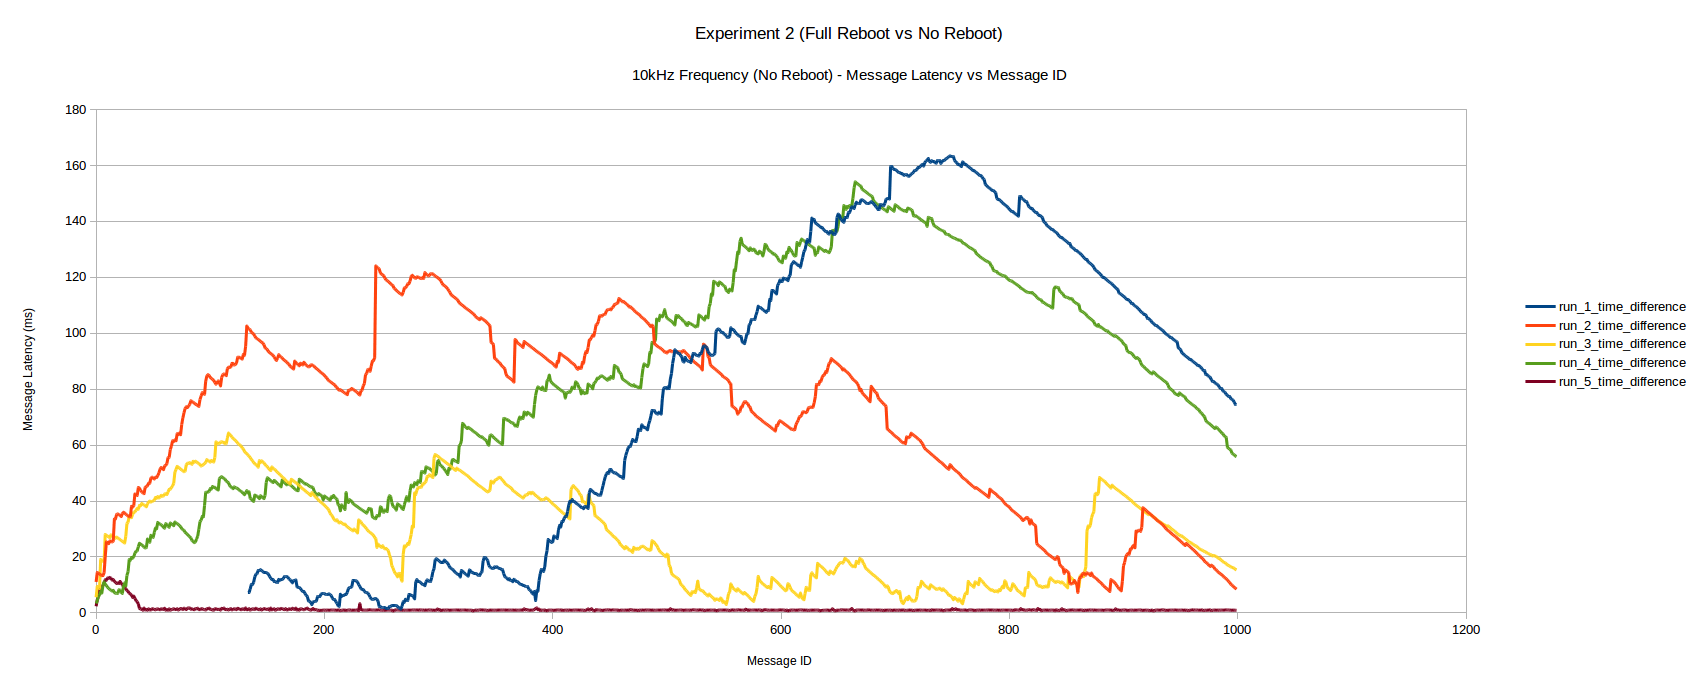
\includegraphics[width=\textwidth]{images/no-reboot-10khz.png}
\caption{Experiment 2 - No Reboot 10KHz Message Frequency}
\label{exp2-noreboot-10khz}
\end{figure}

\begin{figure}
\centering
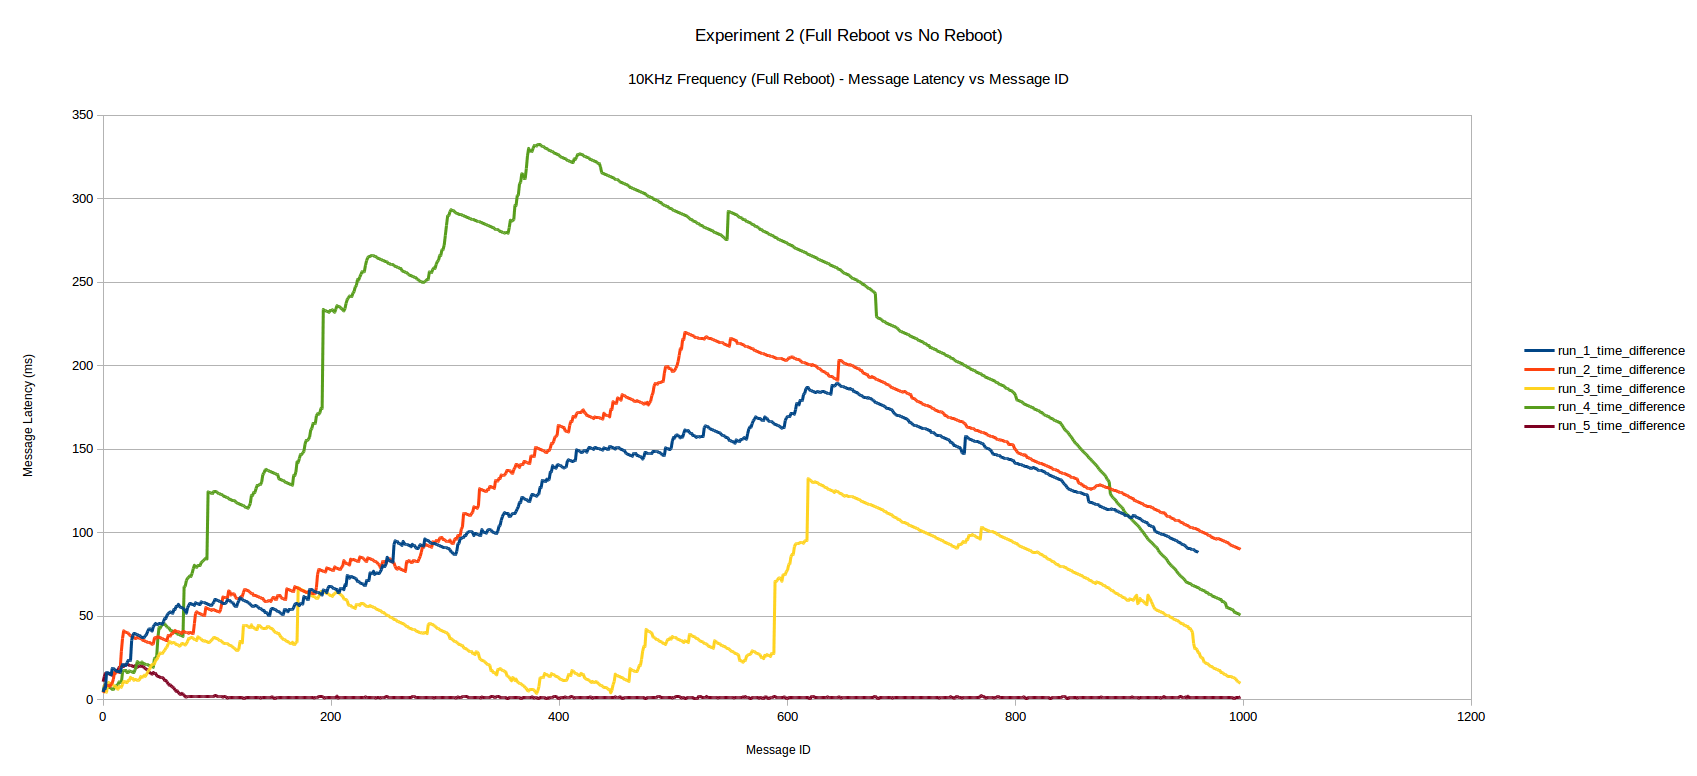
\includegraphics[width=\textwidth]{images/full-reboot-10khz.png}
\caption{Experiment 2 - Full Reboot 10KHz Message Frequency}
\label{exp2-fullreboot-10khz}
\end{figure}

\chapter{Code}

\section{Experiment 1 - Initial Code}
\label{Exp1InitCode}

\subsection{Sender and Receiver}

\begin{lstlisting}[language=Python]
#!/usr/bin/env python

import rospy
from rosberry_experiments.msg import StampedMessage
import time
import sys

N = None
RATE = None
f = None

def listener(msg):
    recv_time = rospy.get_rostime()
    send_time = msg.t

    f.write(str(msg.id))
    f.write(",")
    f.write(str(send_time))
    f.write(",")
    f.write(str(recv_time))
    f.write("\n")

def talker():
    pub = rospy.Publisher('chatter_m', StampedMessage, queue_size=RATE)
    rospy.init_node('talker', anonymous=True)
    rate = rospy.Rate(RATE)
    for i in xrange(N):
        hello_str = "hello world"
        timestamp = rospy.get_rostime()
        pub.publish(id=i, t=timestamp ,message=hello_str )
        rate.sleep()

def main():
    global RATE, N, f
    RATE = int(sys.argv[1])
    N = int(sys.argv[2])
    f = open("times_"+str(RATE)+".txt", "w+")
    print RATE, N
    try:
        sub = rospy.Subscriber("chatter_s", StampedMessage, listener)
        talker()
        rospy.sleep(5)
        f.close()
    except rospy.ROSInterruptException:
        pass


if __name__ == '__main__':
    main()
\end{lstlisting}

\subsection{Echoer}
\begin{lstlisting}[language=Python]
#!/usr/bin/env python

import rospy
from rosberry_experiments.msg import StampedMessage
import time
import sys

RATE = None

def listener(msg, args):
    rate = rospy.Rate(RATE)
    pub = args[0]
    pub.publish(msg)
    rate.sleep()

def main():
    global RATE
    RATE = int(sys.argv[1])
    try:
        rospy.init_node('talker1', anonymous=True)
        pub = rospy.Publisher('chatter_s', StampedMessage, queue_size=RATE)
        sub = rospy.Subscriber("chatter_m", StampedMessage, listener, callback_args=[pub])
        rospy.spin()
    except rospy.ROSInterruptException:
        pass

if __name__ == '__main__':
    main()
\end{lstlisting}

\section{Experiment 1 - Revised Code}

\subsection{Sender and Receiver}
\begin{lstlisting}[language=Python]
#!/usr/bin/env python

import rospy
from rosberry_experiments.msg import StampedMessage
import time
import sys

N = None
RATE = None
f = None

def listener(msg):
    recv_time = rospy.get_rostime()
    sent_time = msg.t
    f.write(str(msg.id) + "," + str(sent_time) + "," + str(recv_time) + "\n")

def talker():
    pub = rospy.Publisher('chatter_m', StampedMessage, queue_size=N)
    rospy.init_node('talker', anonymous=True)
    rate = rospy.Rate(RATE)
    for i in xrange(N):
        hello_str = "hello world"
        timestamp = rospy.get_rostime()
        pub.publish(id=i, t=timestamp, message=hello_str )

        rate.sleep()

def main():
    global RATE, N, f
    RATE = int(sys.argv[1])
    N = int(sys.argv[2])
    f = open("times_"+str(RATE)+".txt", "w+")
    print RATE, N
    try:
        sub = rospy.Subscriber("chatter_s", StampedMessage, listener)
        talker()
        rospy.sleep(5)
        f.close()

    except rospy.ROSInterruptException:
        print "Exception: ROSInterruptException"


if __name__ == '__main__':
    main()
\end{lstlisting}

\subsection{Echoer}
\begin{lstlisting}[language=Python]
#!/usr/bin/env python

import rospy
from rosberry_experiments.msg import StampedMessage
import time
import sys

def listener(msg, args):
    pub = args[0]
    pub.publish(msg)

def main():
    N = int(sys.argv[2])
    rospy.init_node('talker1', anonymous=True)
    pub = rospy.Publisher('chatter_s',
						StampedMessage, queue_size=N)

    sub = rospy.Subscriber("chatter_m",
						StampedMessage, listener, callback_args=[pub])
    try:
        rospy.spin()
    except rospy.ROSInterruptException:
        print "Exception: ROSInterruptException"

if __name__ == '__main__':
    main()
\end{lstlisting}

\chapter{Running the Programs}

To compile this dissertation:
\begin{verbatim}

	> pdflatex dissertation
	> bibtex dissertation
	> pdflatex dissertation
    > pdflatex dissertation

\end{verbatim}


An example of running from the command line is as follows:
\begin{verbatim}
	> rosrun rosberry_experiments run_experiment.py
\end{verbatim}


\chapter{Generating Random Graphs (Example Appendix)}
\label{sec:randomGraph}

\begin{verbatim}
	> java RandomGraph 100 0.9 > 100-90-00.clq
\end{verbatim}
\end{appendices}

%%%%%%%%%%%%%%%%%%%%
%   BIBLIOGRAPHY   %
%%%%%%%%%%%%%%%%%%%%

\bibliographystyle{plain}
\bibliography{bib}

\end{document}
